\documentclass[1p]{elsarticle_modified}
%\bibliographystyle{elsarticle-num}

%\usepackage[colorlinks]{hyperref}
%\usepackage{abbrmath_seonhwa} %\Abb, \Ascr, \Acal ,\Abf, \Afrak
\usepackage{amsfonts}
\usepackage{amssymb}
\usepackage{amsmath}
\usepackage{amsthm}
\usepackage{scalefnt}
\usepackage{amsbsy}
\usepackage{kotex}
\usepackage{caption}
\usepackage{subfig}
\usepackage{color}
\usepackage{graphicx}
\usepackage{xcolor} %% white, black, red, green, blue, cyan, magenta, yellow
\usepackage{float}
\usepackage{setspace}
\usepackage{hyperref}

\usepackage{tikz}
\usetikzlibrary{arrows}

\usepackage{multirow}
\usepackage{array} % fixed length table
\usepackage{hhline}

%%%%%%%%%%%%%%%%%%%%%
\makeatletter
\renewcommand*\env@matrix[1][\arraystretch]{%
	\edef\arraystretch{#1}%
	\hskip -\arraycolsep
	\let\@ifnextchar\new@ifnextchar
	\array{*\c@MaxMatrixCols c}}
\makeatother %https://tex.stackexchange.com/questions/14071/how-can-i-increase-the-line-spacing-in-a-matrix
%%%%%%%%%%%%%%%

\usepackage[normalem]{ulem}

\newcommand{\msout}[1]{\ifmmode\text{\sout{\ensuremath{#1}}}\else\sout{#1}\fi}
%SOURCE: \msout is \stkout macro in https://tex.stackexchange.com/questions/20609/strikeout-in-math-mode

\newcommand{\cancel}[1]{
	\ifmmode
	{\color{red}\msout{#1}}
	\else
	{\color{red}\sout{#1}}
	\fi
}

\newcommand{\add}[1]{
	{\color{blue}\uwave{#1}}
}

\newcommand{\replace}[2]{
	\ifmmode
	{\color{red}\msout{#1}}{\color{blue}\uwave{#2}}
	\else
	{\color{red}\sout{#1}}{\color{blue}\uwave{#2}}
	\fi
}

\newcommand{\Sol}{\mathcal{S}} %segment
\newcommand{\D}{D} %diagram
\newcommand{\A}{\mathcal{A}} %arc


%%%%%%%%%%%%%%%%%%%%%%%%%%%%%5 test

\def\sl{\operatorname{\textup{SL}}(2,\Cbb)}
\def\psl{\operatorname{\textup{PSL}}(2,\Cbb)}
\def\quan{\mkern 1mu \triangleright \mkern 1mu}

\theoremstyle{definition}
\newtheorem{thm}{Theorem}[section]
\newtheorem{prop}[thm]{Proposition}
\newtheorem{lem}[thm]{Lemma}
\newtheorem{ques}[thm]{Question}
\newtheorem{cor}[thm]{Corollary}
\newtheorem{defn}[thm]{Definition}
\newtheorem{exam}[thm]{Example}
\newtheorem{rmk}[thm]{Remark}
\newtheorem{alg}[thm]{Algorithm}

\newcommand{\I}{\sqrt{-1}}
\begin{document}

%\begin{frontmatter}
%
%\title{Boundary parabolic representations of knots up to 8 crossings}
%
%%% Group authors per affiliation:
%\author{Yunhi Cho} 
%\address{Department of Mathematics, University of Seoul, Seoul, Korea}
%\ead{yhcho@uos.ac.kr}
%
%
%\author{Seonhwa Kim} %\fnref{s_kim}}
%\address{Center for Geometry and Physics, Institute for Basic Science, Pohang, 37673, Korea}
%\ead{ryeona17@ibs.re.kr}
%
%\author{Hyuk Kim}
%\address{Department of Mathematical Sciences, Seoul National University, Seoul 08826, Korea}
%\ead{hyukkim@snu.ac.kr}
%
%\author{Seokbeom Yoon}
%\address{Department of Mathematical Sciences, Seoul National University, Seoul, 08826,  Korea}
%\ead{sbyoon15@snu.ac.kr}
%
%\begin{abstract}
%We find all boundary parabolic representation of knots up to 8 crossings.
%
%\end{abstract}
%\begin{keyword}
%    \MSC[2010] 57M25 
%\end{keyword}
%
%\end{frontmatter}

%\linenumbers
%\tableofcontents
%
\newcommand\colored[1]{\textcolor{white}{\rule[-0.35ex]{0.8em}{1.4ex}}\kern-0.8em\color{red} #1}%
%\newcommand\colored[1]{\textcolor{white}{ #1}\kern-2.17ex	\textcolor{white}{ #1}\kern-1.81ex	\textcolor{white}{ #1}\kern-2.15ex\color{red}#1	}

{\Large $\underline{11n_{136}~(K11n_{136})}$}

\setlength{\tabcolsep}{10pt}
\renewcommand{\arraystretch}{1.6}
\vspace{1cm}\begin{tabular}{m{100pt}>{\centering\arraybackslash}m{274pt}}
\multirow{5}{120pt}{
	\centering
	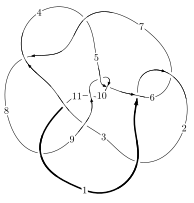
\includegraphics[width=112pt]{../../../GIT/diagram.site/Diagrams/png/752_11n_136.png}\\
\ \ \ A knot diagram\footnotemark}&
\allowdisplaybreaks
\textbf{Linearized knot diagam} \\
\cline{2-2}
 &
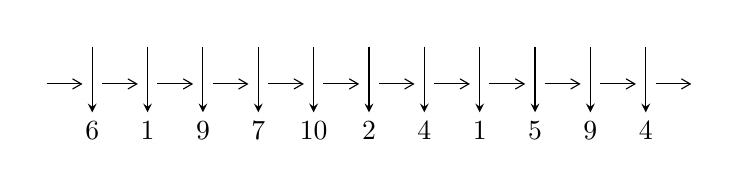
\begin{tikzpicture}[x=20pt, y=17pt]
	% nodes
	\node (C0) at (0, 0) {};
	\node (C1) at (1, 0) {};
	\node (C1U) at (1, +1) {};
	\node (C1D) at (1, -1) {6};

	\node (C2) at (2, 0) {};
	\node (C2U) at (2, +1) {};
	\node (C2D) at (2, -1) {1};

	\node (C3) at (3, 0) {};
	\node (C3U) at (3, +1) {};
	\node (C3D) at (3, -1) {9};

	\node (C4) at (4, 0) {};
	\node (C4U) at (4, +1) {};
	\node (C4D) at (4, -1) {7};

	\node (C5) at (5, 0) {};
	\node (C5U) at (5, +1) {};
	\node (C5D) at (5, -1) {10};

	\node (C6) at (6, 0) {};
	\node (C6U) at (6, +1) {};
	\node (C6D) at (6, -1) {2};

	\node (C7) at (7, 0) {};
	\node (C7U) at (7, +1) {};
	\node (C7D) at (7, -1) {4};

	\node (C8) at (8, 0) {};
	\node (C8U) at (8, +1) {};
	\node (C8D) at (8, -1) {1};

	\node (C9) at (9, 0) {};
	\node (C9U) at (9, +1) {};
	\node (C9D) at (9, -1) {5};

	\node (C10) at (10, 0) {};
	\node (C10U) at (10, +1) {};
	\node (C10D) at (10, -1) {9};

	\node (C11) at (11, 0) {};
	\node (C11U) at (11, +1) {};
	\node (C11D) at (11, -1) {4};
	\node (C12) at (12, 0) {};

	% arrows
	\draw[->,>={angle 60}]
	(C0) edge (C1) (C1) edge (C2) (C2) edge (C3) (C3) edge (C4) (C4) edge (C5) (C5) edge (C6) (C6) edge (C7) (C7) edge (C8) (C8) edge (C9) (C9) edge (C10) (C10) edge (C11) (C11) edge (C12) ;	\draw[->,>=stealth]
	(C1U) edge (C1D) (C2U) edge (C2D) (C3U) edge (C3D) (C4U) edge (C4D) (C5U) edge (C5D) (C6U) edge (C6D) (C7U) edge (C7D) (C8U) edge (C8D) (C9U) edge (C9D) (C10U) edge (C10D) (C11U) edge (C11D) ;
	\end{tikzpicture} \\
\hhline{~~} \\& 
\textbf{Solving Sequence} \\ \cline{2-2} 
 &
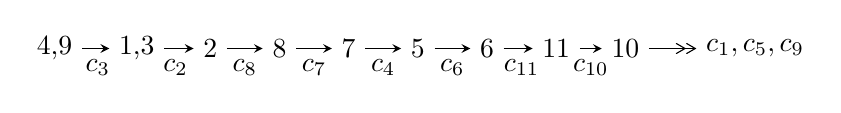
\begin{tikzpicture}[x=25pt, y=7pt]
	% node
	\node (A0) at (-1/8, 0) {4,9};
	\node (A1) at (17/16, 0) {1,3};
	\node (A2) at (17/8, 0) {2};
	\node (A3) at (25/8, 0) {8};
	\node (A4) at (33/8, 0) {7};
	\node (A5) at (41/8, 0) {5};
	\node (A6) at (49/8, 0) {6};
	\node (A7) at (57/8, 0) {11};
	\node (A8) at (65/8, 0) {10};
	\node (C1) at (1/2, -1) {$c_{3}$};
	\node (C2) at (13/8, -1) {$c_{2}$};
	\node (C3) at (21/8, -1) {$c_{8}$};
	\node (C4) at (29/8, -1) {$c_{7}$};
	\node (C5) at (37/8, -1) {$c_{4}$};
	\node (C6) at (45/8, -1) {$c_{6}$};
	\node (C7) at (53/8, -1) {$c_{11}$};
	\node (C8) at (61/8, -1) {$c_{10}$};
	\node (A9) at (10, 0) {$c_{1},c_{5},c_{9}$};

	% edge
	\draw[->,>=stealth]	
	(A0) edge (A1) (A1) edge (A2) (A2) edge (A3) (A3) edge (A4) (A4) edge (A5) (A5) edge (A6) (A6) edge (A7) (A7) edge (A8) ;
	\draw[->>,>={angle 60}]	
	(A8) edge (A9);
\end{tikzpicture} \\ 

\end{tabular} \\

\footnotetext{
The image of knot diagram is generated by the software ``\textbf{Draw programme}" developed by Andrew Bartholomew(\url{http://www.layer8.co.uk/maths/draw/index.htm\#Running-draw}), where we modified some parts for our purpose(\url{https://github.com/CATsTAILs/LinksPainter}).
}\phantom \\ \newline 
\centering \textbf{Ideals for irreducible components\footnotemark of $X_{\text{par}}$} 
 
\begin{align*}
I^u_{1}&=\langle 
83 u^{11}-937 u^{10}+\cdots+244 b-1872,\;-234 u^{11}+2491 u^{10}+\cdots+244 a+6946,\\
\phantom{I^u_{1}}&\phantom{= \langle  }u^{12}-11 u^{11}+57 u^{10}-189 u^9+459 u^8-868 u^7+1293 u^6-1499 u^5+1327 u^4-863 u^3+374 u^2-88 u+8\rangle \\
I^u_{2}&=\langle 
-6 u^{14}-27 u^{13}+\cdots+8 b-31,\;-93 u^{14} a+31 u^{14}+\cdots-303 a+110,\;u^{15}+5 u^{14}+\cdots+8 u+3\rangle \\
I^u_{3}&=\langle 
u^5+2 u^4+u^3+2 u^2+b+u+1,\;- u^5- u^4+u^3-2 u^2+a,\;u^6+2 u^5+u^4+3 u^3+2 u^2+u+1\rangle \\
I^u_{4}&=\langle 
a u+b+1,\;u^2 a+a^2- a u-1,\;u^3- u^2-1\rangle \\
\\
I^v_{1}&=\langle 
a,\;b-1,\;v-1\rangle \\
\end{align*}
\raggedright * 5 irreducible components of $\dim_{\mathbb{C}}=0$, with total 55 representations.\\
\footnotetext{All coefficients of polynomials are rational numbers. But the coefficients are sometimes approximated in decimal forms when there is not enough margin.}
\newpage
\renewcommand{\arraystretch}{1}
\centering \section*{I. $I^u_{1}= \langle 83 u^{11}-937 u^{10}+\cdots+244 b-1872,\;-234 u^{11}+2491 u^{10}+\cdots+244 a+6946,\;u^{12}-11 u^{11}+\cdots-88 u+8 \rangle$}
\flushleft \textbf{(i) Arc colorings}\\
\begin{tabular}{m{7pt} m{180pt} m{7pt} m{180pt} }
\flushright $a_{4}=$&$\begin{pmatrix}1\\0\end{pmatrix}$ \\
\flushright $a_{9}=$&$\begin{pmatrix}0\\u\end{pmatrix}$ \\
\flushright $a_{1}=$&$\begin{pmatrix}0.959016 u^{11}-10.2090 u^{10}+\cdots+186.193 u-28.4672\\-0.340164 u^{11}+3.84016 u^{10}+\cdots-55.9262 u+7.67213\end{pmatrix}$ \\
\flushright $a_{3}=$&$\begin{pmatrix}1\\- u^2\end{pmatrix}$ \\
\flushright $a_{2}=$&$\begin{pmatrix}-1.08402 u^{11}+11.3340 u^{10}+\cdots-191.693 u+29.4672\\0.590164 u^{11}-6.09016 u^{10}+\cdots+66.9262 u-8.67213\end{pmatrix}$ \\
\flushright $a_{8}=$&$\begin{pmatrix}-0.518443 u^{11}+6.26844 u^{10}+\cdots-204.701 u+32.6148\\-0.565574 u^{11}+5.06557 u^{10}+\cdots+14.0082 u-4.14754\end{pmatrix}$ \\
\flushright $a_{7}=$&$\begin{pmatrix}-1.08402 u^{11}+11.3340 u^{10}+\cdots-190.693 u+28.4672\\-0.565574 u^{11}+5.06557 u^{10}+\cdots+14.0082 u-4.14754\end{pmatrix}$ \\
\flushright $a_{5}=$&$\begin{pmatrix}0.485656 u^{11}-5.98566 u^{10}+\cdots+195.705 u-29.6885\\1.16803 u^{11}-11.1680 u^{10}+\cdots+35.8852 u-0.934426\end{pmatrix}$ \\
\flushright $a_{6}=$&$\begin{pmatrix}-0.309426 u^{11}+2.55943 u^{10}+\cdots+27.7418 u-4.85246\\0.598361 u^{11}-5.59836 u^{10}+\cdots+39.7377 u-4.27869\end{pmatrix}$ \\
\flushright $a_{11}=$&$\begin{pmatrix}0.618852 u^{11}-6.36885 u^{10}+\cdots+130.266 u-20.7951\\-0.340164 u^{11}+3.84016 u^{10}+\cdots-55.9262 u+7.67213\end{pmatrix}$ \\
\flushright $a_{10}=$&$\begin{pmatrix}0.618852 u^{11}-6.36885 u^{10}+\cdots+130.266 u-20.7951\\-1.22541 u^{11}+11.7254 u^{10}+\cdots-89.5656 u+11.1803\end{pmatrix}$\\ \flushright $a_{10}=$&$\begin{pmatrix}0.618852 u^{11}-6.36885 u^{10}+\cdots+130.266 u-20.7951\\-1.22541 u^{11}+11.7254 u^{10}+\cdots-89.5656 u+11.1803\end{pmatrix}$\\&\end{tabular}
\flushleft \textbf{(ii) Obstruction class $= -1$}\\~\\
\flushleft \textbf{(iii) Cusp Shapes $= -\frac{69}{61} u^{11}+\frac{679}{61} u^{10}-\frac{3121}{61} u^9+\frac{9220}{61} u^8-\frac{20174}{61} u^7+\frac{34320}{61} u^6-\frac{44856}{61} u^5+\frac{43929}{61} u^4-\frac{31083}{61} u^3+\frac{14067}{61} u^2-\frac{2500}{61} u-\frac{994}{61}$}\\~\\
\newpage\renewcommand{\arraystretch}{1}
\flushleft \textbf{(iv) u-Polynomials at the component}\newline \\
\begin{tabular}{m{50pt}|m{274pt}}
Crossings & \hspace{64pt}u-Polynomials at each crossing \\
\hline $$\begin{aligned}c_{1},c_{5},c_{6}\\c_{9}\end{aligned}$$&$\begin{aligned}
&u^{12}+u^{11}+\cdots-2 u-1
\end{aligned}$\\
\hline $$\begin{aligned}c_{2},c_{10}\end{aligned}$$&$\begin{aligned}
&u^{12}+7 u^{11}+\cdots+8 u+1
\end{aligned}$\\
\hline $$\begin{aligned}c_{3}\end{aligned}$$&$\begin{aligned}
&u^{12}+11 u^{11}+\cdots+88 u+8
\end{aligned}$\\
\hline $$\begin{aligned}c_{4},c_{7}\end{aligned}$$&$\begin{aligned}
&u^{12}-7 u^{11}+\cdots+4 u-8
\end{aligned}$\\
\hline $$\begin{aligned}c_{8},c_{11}\end{aligned}$$&$\begin{aligned}
&u^{12}-2 u^{11}+\cdots+3 u+1
\end{aligned}$\\
\hline
\end{tabular}\\~\\
\newpage\renewcommand{\arraystretch}{1}
\flushleft \textbf{(v) Riley Polynomials at the component}\newline \\
\begin{tabular}{m{50pt}|m{274pt}}
Crossings & \hspace{64pt}Riley Polynomials at each crossing \\
\hline $$\begin{aligned}c_{1},c_{5},c_{6}\\c_{9}\end{aligned}$$&$\begin{aligned}
&y^{12}-7 y^{11}+\cdots-8 y+1
\end{aligned}$\\
\hline $$\begin{aligned}c_{2},c_{10}\end{aligned}$$&$\begin{aligned}
&y^{12}+y^{11}+\cdots-32 y+1
\end{aligned}$\\
\hline $$\begin{aligned}c_{3}\end{aligned}$$&$\begin{aligned}
&y^{12}-7 y^{11}+\cdots-1760 y+64
\end{aligned}$\\
\hline $$\begin{aligned}c_{4},c_{7}\end{aligned}$$&$\begin{aligned}
&y^{12}+5 y^{11}+\cdots-656 y+64
\end{aligned}$\\
\hline $$\begin{aligned}c_{8},c_{11}\end{aligned}$$&$\begin{aligned}
&y^{12}-18 y^{11}+\cdots-21 y+1
\end{aligned}$\\
\hline
\end{tabular}\\~\\
\newpage\flushleft \textbf{(vi) Complex Volumes and Cusp Shapes}
$$\begin{array}{c|c|c}  
\text{Solutions to }I^u_{1}& \I (\text{vol} + \sqrt{-1}CS) & \text{Cusp shape}\\
 \hline 
\begin{aligned}
u &= \phantom{-}0.302190 + 1.082960 I \\
a &= -0.173842 - 0.404485 I \\
b &= -0.385507 + 0.310495 I\end{aligned}
 & \phantom{-}2.70102 - 2.45198 I & -9.00502 + 1.91716 I \\ \hline\begin{aligned}
u &= \phantom{-}0.302190 - 1.082960 I \\
a &= -0.173842 + 0.404485 I \\
b &= -0.385507 - 0.310495 I\end{aligned}
 & \phantom{-}2.70102 + 2.45198 I & -9.00502 - 1.91716 I \\ \hline\begin{aligned}
u &= \phantom{-}1.48047 + 0.22618 I \\
a &= -1.025210 - 0.103256 I \\
b &= \phantom{-}1.49443 + 0.38475 I\end{aligned}
 & -1.76862 - 2.36514 I & -8.64736 + 0.93899 I \\ \hline\begin{aligned}
u &= \phantom{-}1.48047 - 0.22618 I \\
a &= -1.025210 + 0.103256 I \\
b &= \phantom{-}1.49443 - 0.38475 I\end{aligned}
 & -1.76862 + 2.36514 I & -8.64736 - 0.93899 I \\ \hline\begin{aligned}
u &= \phantom{-}0.360681\phantom{ +0.000000I} \\
a &= -0.734365\phantom{ +0.000000I} \\
b &= \phantom{-}0.264871\phantom{ +0.000000I}\end{aligned}
 & -0.612207\phantom{ +0.000000I} & -16.2730\phantom{ +0.000000I} \\ \hline\begin{aligned}
u &= -0.06599 + 1.68520 I \\
a &= -0.168168 + 0.408954 I \\
b &= \phantom{-}0.678073 + 0.310386 I\end{aligned}
 & -1.13692 + 4.86316 I & -15.3188 - 3.9545 I \\ \hline\begin{aligned}
u &= -0.06599 - 1.68520 I \\
a &= -0.168168 - 0.408954 I \\
b &= \phantom{-}0.678073 - 0.310386 I\end{aligned}
 & -1.13692 - 4.86316 I & -15.3188 + 3.9545 I \\ \hline\begin{aligned}
u &= \phantom{-}1.60414 + 0.72863 I \\
a &= \phantom{-}0.881126 - 0.421215 I \\
b &= -1.72036 + 0.03367 I\end{aligned}
 & -9.15791 - 5.54846 I & -14.9776 + 4.7158 I \\ \hline\begin{aligned}
u &= \phantom{-}1.60414 - 0.72863 I \\
a &= \phantom{-}0.881126 + 0.421215 I \\
b &= -1.72036 - 0.03367 I\end{aligned}
 & -9.15791 + 5.54846 I & -14.9776 - 4.7158 I \\ \hline\begin{aligned}
u &= \phantom{-}0.222519\phantom{ +0.000000I} \\
a &= -5.14860\phantom{ +0.000000I} \\
b &= \phantom{-}1.14566\phantom{ +0.000000I}\end{aligned}
 & -4.93861\phantom{ +0.000000I} & -18.1860\phantom{ +0.000000I}\\
 \hline 
 \end{array}$$\newpage$$\begin{array}{c|c|c}  
\text{Solutions to }I^u_{1}& \I (\text{vol} + \sqrt{-1}CS) & \text{Cusp shape}\\
 \hline 
\begin{aligned}
u &= \phantom{-}1.88759 + 0.64713 I \\
a &= \phantom{-}0.927570 - 0.032494 I \\
b &= -1.77190 - 0.53892 I\end{aligned}
 & -7.6014 - 13.7948 I & -13.8218 + 7.4992 I \\ \hline\begin{aligned}
u &= \phantom{-}1.88759 - 0.64713 I \\
a &= \phantom{-}0.927570 + 0.032494 I \\
b &= -1.77190 + 0.53892 I\end{aligned}
 & -7.6014 + 13.7948 I & -13.8218 - 7.4992 I\\
 \hline 
 \end{array}$$\newpage\newpage\renewcommand{\arraystretch}{1}
\centering \section*{II. $I^u_{2}= \langle -6 u^{14}-27 u^{13}+\cdots+8 b-31,\;-93 u^{14} a+31 u^{14}+\cdots-303 a+110,\;u^{15}+5 u^{14}+\cdots+8 u+3 \rangle$}
\flushleft \textbf{(i) Arc colorings}\\
\begin{tabular}{m{7pt} m{180pt} m{7pt} m{180pt} }
\flushright $a_{4}=$&$\begin{pmatrix}1\\0\end{pmatrix}$ \\
\flushright $a_{9}=$&$\begin{pmatrix}0\\u\end{pmatrix}$ \\
\flushright $a_{1}=$&$\begin{pmatrix}a\\\frac{3}{4} u^{14}+\frac{27}{8} u^{13}+\cdots+\frac{49}{8} u+\frac{31}{8}\end{pmatrix}$ \\
\flushright $a_{3}=$&$\begin{pmatrix}1\\- u^2\end{pmatrix}$ \\
\flushright $a_{2}=$&$\begin{pmatrix}-0.375000 a u^{14}-0.0833333 u^{14}+\cdots-2.25000 a+0.708333\\\frac{3}{8} u^{14} a-\frac{5}{4} u^{14}+\cdots+\frac{9}{4} a-3\end{pmatrix}$ \\
\flushright $a_{8}=$&$\begin{pmatrix}-0.750000 a u^{14}+0.333333 u^{14}+\cdots-3.87500 a+1.29167\\-\frac{1}{4} u^{14}-\frac{9}{8} u^{13}+\cdots-\frac{3}{8} u-1\end{pmatrix}$ \\
\flushright $a_{7}=$&$\begin{pmatrix}-0.750000 a u^{14}+0.0833333 u^{14}+\cdots-3.87500 a+0.291667\\-\frac{1}{4} u^{14}-\frac{9}{8} u^{13}+\cdots-\frac{3}{8} u-1\end{pmatrix}$ \\
\flushright $a_{5}=$&$\begin{pmatrix}\frac{5}{8} u^{14} a+\frac{1}{24} u^{14}+\cdots+\frac{19}{8} a+\frac{31}{12}\\\frac{1}{2} u^{14}+\frac{19}{8} u^{13}+\cdots+\frac{33}{8} u+\frac{17}{8}\end{pmatrix}$ \\
\flushright $a_{6}=$&$\begin{pmatrix}\frac{1}{4} u^{14} a-\frac{31}{24} u^{14}+\cdots+2 a-\frac{101}{24}\\\frac{1}{4} u^{13} a-\frac{1}{4} u^{14}+\cdots+\frac{3}{8} a-\frac{1}{8}\end{pmatrix}$ \\
\flushright $a_{11}=$&$\begin{pmatrix}\frac{3}{4} u^{14}+\frac{27}{8} u^{13}+\cdots+a+\frac{31}{8}\\\frac{3}{4} u^{14}+\frac{27}{8} u^{13}+\cdots+\frac{49}{8} u+\frac{31}{8}\end{pmatrix}$ \\
\flushright $a_{10}=$&$\begin{pmatrix}\frac{3}{4} u^{14}+\frac{27}{8} u^{13}+\cdots+a+\frac{31}{8}\\\frac{1}{2} u^{14}+\frac{19}{8} u^{13}+\cdots+\frac{43}{8} u+\frac{11}{4}\end{pmatrix}$\\ \flushright $a_{10}=$&$\begin{pmatrix}\frac{3}{4} u^{14}+\frac{27}{8} u^{13}+\cdots+a+\frac{31}{8}\\\frac{1}{2} u^{14}+\frac{19}{8} u^{13}+\cdots+\frac{43}{8} u+\frac{11}{4}\end{pmatrix}$\\&\end{tabular}
\flushleft \textbf{(ii) Obstruction class $= -1$}\\~\\
\flushleft \textbf{(iii) Cusp Shapes $= 4 u^{14}+16 u^{13}-\frac{15}{2} u^{12}-115 u^{11}-131 u^{10}+156 u^9+\frac{857}{2} u^8+263 u^7-94 u^6-193 u^5-58 u^4+21 u^3+16 u^2+28 u+\frac{3}{2}$}\\~\\
\newpage\renewcommand{\arraystretch}{1}
\flushleft \textbf{(iv) u-Polynomials at the component}\newline \\
\begin{tabular}{m{50pt}|m{274pt}}
Crossings & \hspace{64pt}u-Polynomials at each crossing \\
\hline $$\begin{aligned}c_{1},c_{5},c_{6}\\c_{9}\end{aligned}$$&$\begin{aligned}
&u^{30}- u^{29}+\cdots+2 u^2+1
\end{aligned}$\\
\hline $$\begin{aligned}c_{2},c_{10}\end{aligned}$$&$\begin{aligned}
&u^{30}+17 u^{29}+\cdots-4 u+1
\end{aligned}$\\
\hline $$\begin{aligned}c_{3}\end{aligned}$$&$\begin{aligned}
&(u^{15}-5 u^{14}+\cdots+8 u-3)^{2}
\end{aligned}$\\
\hline $$\begin{aligned}c_{4},c_{7}\end{aligned}$$&$\begin{aligned}
&(u^{15}+3 u^{14}+\cdots+5 u+1)^{2}
\end{aligned}$\\
\hline $$\begin{aligned}c_{8},c_{11}\end{aligned}$$&$\begin{aligned}
&u^{30}-2 u^{29}+\cdots+66 u-79
\end{aligned}$\\
\hline
\end{tabular}\\~\\
\newpage\renewcommand{\arraystretch}{1}
\flushleft \textbf{(v) Riley Polynomials at the component}\newline \\
\begin{tabular}{m{50pt}|m{274pt}}
Crossings & \hspace{64pt}Riley Polynomials at each crossing \\
\hline $$\begin{aligned}c_{1},c_{5},c_{6}\\c_{9}\end{aligned}$$&$\begin{aligned}
&y^{30}-17 y^{29}+\cdots+4 y+1
\end{aligned}$\\
\hline $$\begin{aligned}c_{2},c_{10}\end{aligned}$$&$\begin{aligned}
&y^{30}-5 y^{29}+\cdots-112 y+1
\end{aligned}$\\
\hline $$\begin{aligned}c_{3}\end{aligned}$$&$\begin{aligned}
&(y^{15}-21 y^{14}+\cdots-2 y-9)^{2}
\end{aligned}$\\
\hline $$\begin{aligned}c_{4},c_{7}\end{aligned}$$&$\begin{aligned}
&(y^{15}+5 y^{14}+\cdots+7 y-1)^{2}
\end{aligned}$\\
\hline $$\begin{aligned}c_{8},c_{11}\end{aligned}$$&$\begin{aligned}
&y^{30}-30 y^{29}+\cdots-120802 y+6241
\end{aligned}$\\
\hline
\end{tabular}\\~\\
\newpage\flushleft \textbf{(vi) Complex Volumes and Cusp Shapes}
$$\begin{array}{c|c|c}  
\text{Solutions to }I^u_{2}& \I (\text{vol} + \sqrt{-1}CS) & \text{Cusp shape}\\
 \hline 
\begin{aligned}
u &= -0.573512 + 0.780031 I \\
a &= -0.303879 + 1.027660 I \\
b &= -0.674810 + 0.174597 I\end{aligned}
 & \phantom{-}1.85339 - 2.65754 I & -12.13634 + 3.34510 I \\ \hline\begin{aligned}
u &= -0.573512 + 0.780031 I \\
a &= -0.558164 - 0.454721 I \\
b &= \phantom{-}0.627325 + 0.826408 I\end{aligned}
 & \phantom{-}1.85339 - 2.65754 I & -12.13634 + 3.34510 I \\ \hline\begin{aligned}
u &= -0.573512 - 0.780031 I \\
a &= -0.303879 - 1.027660 I \\
b &= -0.674810 - 0.174597 I\end{aligned}
 & \phantom{-}1.85339 + 2.65754 I & -12.13634 - 3.34510 I \\ \hline\begin{aligned}
u &= -0.573512 - 0.780031 I \\
a &= -0.558164 + 0.454721 I \\
b &= \phantom{-}0.627325 - 0.826408 I\end{aligned}
 & \phantom{-}1.85339 + 2.65754 I & -12.13634 - 3.34510 I \\ \hline\begin{aligned}
u &= \phantom{-}0.697369 + 0.218567 I \\
a &= -0.921356 + 0.311277 I \\
b &= \phantom{-}0.314929 + 1.087780 I\end{aligned}
 & \phantom{-}0.330230 + 0.679087 I & -12.40066 - 0.76832 I \\ \hline\begin{aligned}
u &= \phantom{-}0.697369 + 0.218567 I \\
a &= -0.85635 - 1.29144 I \\
b &= \phantom{-}0.710560 - 0.015696 I\end{aligned}
 & \phantom{-}0.330230 + 0.679087 I & -12.40066 - 0.76832 I \\ \hline\begin{aligned}
u &= \phantom{-}0.697369 - 0.218567 I \\
a &= -0.921356 - 0.311277 I \\
b &= \phantom{-}0.314929 - 1.087780 I\end{aligned}
 & \phantom{-}0.330230 - 0.679087 I & -12.40066 + 0.76832 I \\ \hline\begin{aligned}
u &= \phantom{-}0.697369 - 0.218567 I \\
a &= -0.85635 + 1.29144 I \\
b &= \phantom{-}0.710560 + 0.015696 I\end{aligned}
 & \phantom{-}0.330230 - 0.679087 I & -12.40066 + 0.76832 I \\ \hline\begin{aligned}
u &= -0.624643 + 0.305436 I \\
a &= \phantom{-}0.722934 + 0.424315 I \\
b &= \phantom{-}0.23544 + 1.52005 I\end{aligned}
 & -0.89474 - 6.09921 I & -15.4033 + 6.7831 I \\ \hline\begin{aligned}
u &= -0.624643 + 0.305436 I \\
a &= -0.65611 + 2.11265 I \\
b &= \phantom{-}0.581176 + 0.044236 I\end{aligned}
 & -0.89474 - 6.09921 I & -15.4033 + 6.7831 I\\
 \hline 
 \end{array}$$\newpage$$\begin{array}{c|c|c}  
\text{Solutions to }I^u_{2}& \I (\text{vol} + \sqrt{-1}CS) & \text{Cusp shape}\\
 \hline 
\begin{aligned}
u &= -0.624643 - 0.305436 I \\
a &= \phantom{-}0.722934 - 0.424315 I \\
b &= \phantom{-}0.23544 - 1.52005 I\end{aligned}
 & -0.89474 + 6.09921 I & -15.4033 - 6.7831 I \\ \hline\begin{aligned}
u &= -0.624643 - 0.305436 I \\
a &= -0.65611 - 2.11265 I \\
b &= \phantom{-}0.581176 - 0.044236 I\end{aligned}
 & -0.89474 + 6.09921 I & -15.4033 - 6.7831 I \\ \hline\begin{aligned}
u &= \phantom{-}0.067784 + 0.504699 I \\
a &= -0.069426 - 1.144650 I \\
b &= \phantom{-}0.186932 + 0.933368 I\end{aligned}
 & \phantom{-}2.10570 - 2.66884 I & -8.49589 + 5.19452 I \\ \hline\begin{aligned}
u &= \phantom{-}0.067784 + 0.504699 I \\
a &= -1.86545 + 0.11984 I \\
b &= -0.572998 + 0.112628 I\end{aligned}
 & \phantom{-}2.10570 - 2.66884 I & -8.49589 + 5.19452 I \\ \hline\begin{aligned}
u &= \phantom{-}0.067784 - 0.504699 I \\
a &= -0.069426 + 1.144650 I \\
b &= \phantom{-}0.186932 - 0.933368 I\end{aligned}
 & \phantom{-}2.10570 + 2.66884 I & -8.49589 - 5.19452 I \\ \hline\begin{aligned}
u &= \phantom{-}0.067784 - 0.504699 I \\
a &= -1.86545 - 0.11984 I \\
b &= -0.572998 - 0.112628 I\end{aligned}
 & \phantom{-}2.10570 + 2.66884 I & -8.49589 - 5.19452 I \\ \hline\begin{aligned}
u &= -1.49696 + 0.32578 I \\
a &= -0.926351 - 0.253533 I \\
b &= \phantom{-}1.82057 + 0.02441 I\end{aligned}
 & -6.55037 + 0.76607 I & -13.52677 - 0.03940 I \\ \hline\begin{aligned}
u &= -1.49696 + 0.32578 I \\
a &= \phantom{-}1.157790 + 0.268278 I \\
b &= -1.46931 - 0.07774 I\end{aligned}
 & -6.55037 + 0.76607 I & -13.52677 - 0.03940 I \\ \hline\begin{aligned}
u &= -1.49696 - 0.32578 I \\
a &= -0.926351 + 0.253533 I \\
b &= \phantom{-}1.82057 - 0.02441 I\end{aligned}
 & -6.55037 - 0.76607 I & -13.52677 + 0.03940 I \\ \hline\begin{aligned}
u &= -1.49696 - 0.32578 I \\
a &= \phantom{-}1.157790 - 0.268278 I \\
b &= -1.46931 + 0.07774 I\end{aligned}
 & -6.55037 - 0.76607 I & -13.52677 + 0.03940 I\\
 \hline 
 \end{array}$$\newpage$$\begin{array}{c|c|c}  
\text{Solutions to }I^u_{2}& \I (\text{vol} + \sqrt{-1}CS) & \text{Cusp shape}\\
 \hline 
\begin{aligned}
u &= -1.60501\phantom{ +0.000000I} \\
a &= \phantom{-}1.20656\phantom{ +0.000000I} \\
b &= -0.990302\phantom{ +0.000000I}\end{aligned}
 & -7.32542\phantom{ +0.000000I} & -4.72890\phantom{ +0.000000I} \\ \hline\begin{aligned}
u &= -1.60501\phantom{ +0.000000I} \\
a &= -0.617005\phantom{ +0.000000I} \\
b &= \phantom{-}1.93654\phantom{ +0.000000I}\end{aligned}
 & -7.32542\phantom{ +0.000000I} & -4.72890\phantom{ +0.000000I} \\ \hline\begin{aligned}
u &= -1.75343 + 0.35354 I \\
a &= \phantom{-}0.980020 - 0.156747 I \\
b &= -1.65186 + 0.31915 I\end{aligned}
 & -4.38929 + 7.65996 I & -11.60171 - 4.83891 I \\ \hline\begin{aligned}
u &= -1.75343 + 0.35354 I \\
a &= -0.940537 - 0.007624 I \\
b &= \phantom{-}1.66298 - 0.62132 I\end{aligned}
 & -4.38929 + 7.65996 I & -11.60171 - 4.83891 I \\ \hline\begin{aligned}
u &= -1.75343 - 0.35354 I \\
a &= \phantom{-}0.980020 + 0.156747 I \\
b &= -1.65186 - 0.31915 I\end{aligned}
 & -4.38929 - 7.65996 I & -11.60171 + 4.83891 I \\ \hline\begin{aligned}
u &= -1.75343 - 0.35354 I \\
a &= -0.940537 + 0.007624 I \\
b &= \phantom{-}1.66298 + 0.62132 I\end{aligned}
 & -4.38929 - 7.65996 I & -11.60171 + 4.83891 I \\ \hline\begin{aligned}
u &= \phantom{-}1.98590 + 0.14793 I \\
a &= \phantom{-}0.901839 - 0.019745 I \\
b &= -1.45017 + 0.51636 I\end{aligned}
 & -10.17640 + 2.57627 I & -15.0709 - 4.0254 I \\ \hline\begin{aligned}
u &= \phantom{-}1.98590 + 0.14793 I \\
a &= \phantom{-}0.706941 - 0.312672 I \\
b &= -1.79388 - 0.09420 I\end{aligned}
 & -10.17640 + 2.57627 I & -15.0709 - 4.0254 I \\ \hline\begin{aligned}
u &= \phantom{-}1.98590 - 0.14793 I \\
a &= \phantom{-}0.901839 + 0.019745 I \\
b &= -1.45017 - 0.51636 I\end{aligned}
 & -10.17640 - 2.57627 I & -15.0709 + 4.0254 I \\ \hline\begin{aligned}
u &= \phantom{-}1.98590 - 0.14793 I \\
a &= \phantom{-}0.706941 + 0.312672 I \\
b &= -1.79388 + 0.09420 I\end{aligned}
 & -10.17640 - 2.57627 I & -15.0709 + 4.0254 I\\
 \hline 
 \end{array}$$\newpage\newpage\renewcommand{\arraystretch}{1}
\centering \section*{III. $I^u_{3}= \langle u^5+2 u^4+u^3+2 u^2+b+u+1,\;- u^5- u^4+u^3-2 u^2+a,\;u^6+2 u^5+u^4+3 u^3+2 u^2+u+1 \rangle$}
\flushleft \textbf{(i) Arc colorings}\\
\begin{tabular}{m{7pt} m{180pt} m{7pt} m{180pt} }
\flushright $a_{4}=$&$\begin{pmatrix}1\\0\end{pmatrix}$ \\
\flushright $a_{9}=$&$\begin{pmatrix}0\\u\end{pmatrix}$ \\
\flushright $a_{1}=$&$\begin{pmatrix}u^5+u^4- u^3+2 u^2\\- u^5-2 u^4- u^3-2 u^2- u-1\end{pmatrix}$ \\
\flushright $a_{3}=$&$\begin{pmatrix}1\\- u^2\end{pmatrix}$ \\
\flushright $a_{2}=$&$\begin{pmatrix}- u^4-2 u^3- u^2-2 u\\- u^5-2 u^4- u^3-3 u^2- u\end{pmatrix}$ \\
\flushright $a_{8}=$&$\begin{pmatrix}- u^5- u^4+u^3-2 u^2+u\\u^5+2 u^4+u^3+3 u^2+2 u+1\end{pmatrix}$ \\
\flushright $a_{7}=$&$\begin{pmatrix}u^4+2 u^3+u^2+3 u+1\\u^5+2 u^4+u^3+3 u^2+2 u+1\end{pmatrix}$ \\
\flushright $a_{5}=$&$\begin{pmatrix}u^5+2 u^4+u^2+u-1\\u^5+u^4- u^3+2 u^2- u-1\end{pmatrix}$ \\
\flushright $a_{6}=$&$\begin{pmatrix}u^5+2 u^4+u^2+2 u\\u^5+u^4-2 u^3+u^2-1\end{pmatrix}$ \\
\flushright $a_{11}=$&$\begin{pmatrix}- u^4-2 u^3- u-1\\- u^5-2 u^4- u^3-2 u^2- u-1\end{pmatrix}$ \\
\flushright $a_{10}=$&$\begin{pmatrix}- u^4-2 u^3- u-1\\- u^5-3 u^4-3 u^3-3 u^2-2 u-2\end{pmatrix}$\\ \flushright $a_{10}=$&$\begin{pmatrix}- u^4-2 u^3- u-1\\- u^5-3 u^4-3 u^3-3 u^2-2 u-2\end{pmatrix}$\\&\end{tabular}
\flushleft \textbf{(ii) Obstruction class $= 1$}\\~\\
\flushleft \textbf{(iii) Cusp Shapes $= 7 u^5+16 u^4+8 u^3+12 u^2+12 u-5$}\\~\\
\newpage\renewcommand{\arraystretch}{1}
\flushleft \textbf{(iv) u-Polynomials at the component}\newline \\
\begin{tabular}{m{50pt}|m{274pt}}
Crossings & \hspace{64pt}u-Polynomials at each crossing \\
\hline $$\begin{aligned}c_{1},c_{5}\end{aligned}$$&$\begin{aligned}
&u^6-2 u^4+2 u^2+u-1
\end{aligned}$\\
\hline $$\begin{aligned}c_{2},c_{10}\end{aligned}$$&$\begin{aligned}
&u^6+4 u^5+8 u^4+10 u^3+8 u^2+5 u+1
\end{aligned}$\\
\hline $$\begin{aligned}c_{3}\end{aligned}$$&$\begin{aligned}
&u^6+2 u^5+u^4+3 u^3+2 u^2+u+1
\end{aligned}$\\
\hline $$\begin{aligned}c_{4}\end{aligned}$$&$\begin{aligned}
&u^6- u^5+2 u^4-3 u^3+u^2-2 u+1
\end{aligned}$\\
\hline $$\begin{aligned}c_{6},c_{9}\end{aligned}$$&$\begin{aligned}
&u^6-2 u^4+2 u^2- u-1
\end{aligned}$\\
\hline $$\begin{aligned}c_{7}\end{aligned}$$&$\begin{aligned}
&u^6+u^5+2 u^4+3 u^3+u^2+2 u+1
\end{aligned}$\\
\hline $$\begin{aligned}c_{8},c_{11}\end{aligned}$$&$\begin{aligned}
&u^6- u^5- u^4+2 u^3-3 u^2+2 u-1
\end{aligned}$\\
\hline
\end{tabular}\\~\\
\newpage\renewcommand{\arraystretch}{1}
\flushleft \textbf{(v) Riley Polynomials at the component}\newline \\
\begin{tabular}{m{50pt}|m{274pt}}
Crossings & \hspace{64pt}Riley Polynomials at each crossing \\
\hline $$\begin{aligned}c_{1},c_{5},c_{6}\\c_{9}\end{aligned}$$&$\begin{aligned}
&y^6-4 y^5+8 y^4-10 y^3+8 y^2-5 y+1
\end{aligned}$\\
\hline $$\begin{aligned}c_{2},c_{10}\end{aligned}$$&$\begin{aligned}
&y^6-10 y^3-20 y^2-9 y+1
\end{aligned}$\\
\hline $$\begin{aligned}c_{3}\end{aligned}$$&$\begin{aligned}
&y^6-2 y^5-7 y^4-7 y^3+3 y+1
\end{aligned}$\\
\hline $$\begin{aligned}c_{4},c_{7}\end{aligned}$$&$\begin{aligned}
&y^6+3 y^5-7 y^3-7 y^2-2 y+1
\end{aligned}$\\
\hline $$\begin{aligned}c_{8},c_{11}\end{aligned}$$&$\begin{aligned}
&y^6-3 y^5- y^4+4 y^3+3 y^2+2 y+1
\end{aligned}$\\
\hline
\end{tabular}\\~\\
\newpage\flushleft \textbf{(vi) Complex Volumes and Cusp Shapes}
$$\begin{array}{c|c|c}  
\text{Solutions to }I^u_{3}& \I (\text{vol} + \sqrt{-1}CS) & \text{Cusp shape}\\
 \hline 
\begin{aligned}
u &= \phantom{-}0.392638 + 0.978074 I \\
a &= \phantom{-}0.742271 + 0.355591 I \\
b &= -0.056351 + 0.865615 I\end{aligned}
 & \phantom{-}0.69572 + 5.66603 I & -8.99565 - 5.65371 I \\ \hline\begin{aligned}
u &= \phantom{-}0.392638 - 0.978074 I \\
a &= \phantom{-}0.742271 - 0.355591 I \\
b &= -0.056351 - 0.865615 I\end{aligned}
 & \phantom{-}0.69572 - 5.66603 I & -8.99565 + 5.65371 I \\ \hline\begin{aligned}
u &= -0.788940\phantom{ +0.000000I} \\
a &= \phantom{-}1.81768\phantom{ +0.000000I} \\
b &= -1.43404\phantom{ +0.000000I}\end{aligned}
 & -4.14809\phantom{ +0.000000I} & -6.86750\phantom{ +0.000000I} \\ \hline\begin{aligned}
u &= \phantom{-}0.015196 + 0.750196 I \\
a &= -0.759470 + 0.678272 I \\
b &= -0.520377 - 0.559444 I\end{aligned}
 & \phantom{-}3.09094 - 3.67876 I & -6.55000 + 7.14850 I \\ \hline\begin{aligned}
u &= \phantom{-}0.015196 - 0.750196 I \\
a &= -0.759470 - 0.678272 I \\
b &= -0.520377 + 0.559444 I\end{aligned}
 & \phantom{-}3.09094 + 3.67876 I & -6.55000 - 7.14850 I \\ \hline\begin{aligned}
u &= -2.02673\phantom{ +0.000000I} \\
a &= -0.783279\phantom{ +0.000000I} \\
b &= \phantom{-}1.58749\phantom{ +0.000000I}\end{aligned}
 & -10.0050\phantom{ +0.000000I} & -16.0410\phantom{ +0.000000I}\\
 \hline 
 \end{array}$$\newpage\newpage\renewcommand{\arraystretch}{1}
\centering \section*{IV. $I^u_{4}= \langle a u+b+1,\;u^2 a+a^2- a u-1,\;u^3- u^2-1 \rangle$}
\flushleft \textbf{(i) Arc colorings}\\
\begin{tabular}{m{7pt} m{180pt} m{7pt} m{180pt} }
\flushright $a_{4}=$&$\begin{pmatrix}1\\0\end{pmatrix}$ \\
\flushright $a_{9}=$&$\begin{pmatrix}0\\u\end{pmatrix}$ \\
\flushright $a_{1}=$&$\begin{pmatrix}a\\- a u-1\end{pmatrix}$ \\
\flushright $a_{3}=$&$\begin{pmatrix}1\\- u^2\end{pmatrix}$ \\
\flushright $a_{2}=$&$\begin{pmatrix}a u- u^2+u+1\\- a u- u^2\end{pmatrix}$ \\
\flushright $a_{8}=$&$\begin{pmatrix}- a+u\\- u^2+u\end{pmatrix}$ \\
\flushright $a_{7}=$&$\begin{pmatrix}- u^2- a+2 u\\- u^2+u\end{pmatrix}$ \\
\flushright $a_{5}=$&$\begin{pmatrix}u^2 a- a u+u-1\\u-1\end{pmatrix}$ \\
\flushright $a_{6}=$&$\begin{pmatrix}u^2 a- a u- u^2- a+u\\u^2 a- u^2- a+2 u\end{pmatrix}$ \\
\flushright $a_{11}=$&$\begin{pmatrix}- a u+a-1\\- a u-1\end{pmatrix}$ \\
\flushright $a_{10}=$&$\begin{pmatrix}- a u+a-1\\- a u+u^2+a-1\end{pmatrix}$\\ \flushright $a_{10}=$&$\begin{pmatrix}- a u+a-1\\- a u+u^2+a-1\end{pmatrix}$\\&\end{tabular}
\flushleft \textbf{(ii) Obstruction class $= 1$}\\~\\
\flushleft \textbf{(iii) Cusp Shapes $= -4 u^2-4 u-12$}\\~\\
\newpage\renewcommand{\arraystretch}{1}
\flushleft \textbf{(iv) u-Polynomials at the component}\newline \\
\begin{tabular}{m{50pt}|m{274pt}}
Crossings & \hspace{64pt}u-Polynomials at each crossing \\
\hline $$\begin{aligned}c_{1},c_{5}\end{aligned}$$&$\begin{aligned}
&u^6-2 u^4- u^3+2 u^2-1
\end{aligned}$\\
\hline $$\begin{aligned}c_{2},c_{10}\end{aligned}$$&$\begin{aligned}
&u^6+4 u^5+8 u^4+11 u^3+8 u^2+4 u+1
\end{aligned}$\\
\hline $$\begin{aligned}c_{3}\end{aligned}$$&$\begin{aligned}
&(u^3- u^2-1)^2
\end{aligned}$\\
\hline $$\begin{aligned}c_{4}\end{aligned}$$&$\begin{aligned}
&(u^3+u+1)^2
\end{aligned}$\\
\hline $$\begin{aligned}c_{6},c_{9}\end{aligned}$$&$\begin{aligned}
&u^6-2 u^4+u^3+2 u^2-1
\end{aligned}$\\
\hline $$\begin{aligned}c_{7}\end{aligned}$$&$\begin{aligned}
&(u^3+u-1)^2
\end{aligned}$\\
\hline $$\begin{aligned}c_{8},c_{11}\end{aligned}$$&$\begin{aligned}
&u^6-3 u^5+2 u^4+u^3-3 u^2+2 u-1
\end{aligned}$\\
\hline
\end{tabular}\\~\\
\newpage\renewcommand{\arraystretch}{1}
\flushleft \textbf{(v) Riley Polynomials at the component}\newline \\
\begin{tabular}{m{50pt}|m{274pt}}
Crossings & \hspace{64pt}Riley Polynomials at each crossing \\
\hline $$\begin{aligned}c_{1},c_{5},c_{6}\\c_{9}\end{aligned}$$&$\begin{aligned}
&y^6-4 y^5+8 y^4-11 y^3+8 y^2-4 y+1
\end{aligned}$\\
\hline $$\begin{aligned}c_{2},c_{10}\end{aligned}$$&$\begin{aligned}
&y^6-8 y^4-23 y^3-8 y^2+1
\end{aligned}$\\
\hline $$\begin{aligned}c_{3}\end{aligned}$$&$\begin{aligned}
&(y^3- y^2-2 y-1)^2
\end{aligned}$\\
\hline $$\begin{aligned}c_{4},c_{7}\end{aligned}$$&$\begin{aligned}
&(y^3+2 y^2+y-1)^2
\end{aligned}$\\
\hline $$\begin{aligned}c_{8},c_{11}\end{aligned}$$&$\begin{aligned}
&y^6-5 y^5+4 y^4-3 y^3+y^2+2 y+1
\end{aligned}$\\
\hline
\end{tabular}\\~\\
\newpage\flushleft \textbf{(vi) Complex Volumes and Cusp Shapes}
$$\begin{array}{c|c|c}  
\text{Solutions to }I^u_{4}& \I (\text{vol} + \sqrt{-1}CS) & \text{Cusp shape}\\
 \hline 
\begin{aligned}
u &= -0.232786 + 0.792552 I \\
a &= -0.669484 + 0.462841 I \\
b &= -0.789021 + 0.638344 I\end{aligned}
 & \phantom{-}2.21137 - 1.58317 I & -8.77306 - 1.69425 I \\ \hline\begin{aligned}
u &= -0.232786 + 0.792552 I \\
a &= \phantom{-}1.010650 + 0.698701 I \\
b &= -0.210979 - 0.638344 I\end{aligned}
 & \phantom{-}2.21137 - 1.58317 I & -8.77306 - 1.69425 I \\ \hline\begin{aligned}
u &= -0.232786 - 0.792552 I \\
a &= -0.669484 - 0.462841 I \\
b &= -0.789021 - 0.638344 I\end{aligned}
 & \phantom{-}2.21137 + 1.58317 I & -8.77306 + 1.69425 I \\ \hline\begin{aligned}
u &= -0.232786 - 0.792552 I \\
a &= \phantom{-}1.010650 - 0.698701 I \\
b &= -0.210979 + 0.638344 I\end{aligned}
 & \phantom{-}2.21137 + 1.58317 I & -8.77306 + 1.69425 I \\ \hline\begin{aligned}
u &= \phantom{-}1.46557\phantom{ +0.000000I} \\
a &= \phantom{-}0.715431\phantom{ +0.000000I} \\
b &= -2.04852\phantom{ +0.000000I}\end{aligned}
 & -7.71260\phantom{ +0.000000I} & -26.4540\phantom{ +0.000000I} \\ \hline\begin{aligned}
u &= \phantom{-}1.46557\phantom{ +0.000000I} \\
a &= -1.39776\phantom{ +0.000000I} \\
b &= \phantom{-}1.04852\phantom{ +0.000000I}\end{aligned}
 & -7.71260\phantom{ +0.000000I} & -26.4540\phantom{ +0.000000I}\\
 \hline 
 \end{array}$$\newpage\newpage\renewcommand{\arraystretch}{1}
\centering \section*{V. $I^v_{1}= \langle a,\;b-1,\;v-1 \rangle$}
\flushleft \textbf{(i) Arc colorings}\\
\begin{tabular}{m{7pt} m{180pt} m{7pt} m{180pt} }
\flushright $a_{4}=$&$\begin{pmatrix}1\\0\end{pmatrix}$ \\
\flushright $a_{9}=$&$\begin{pmatrix}1\\0\end{pmatrix}$ \\
\flushright $a_{1}=$&$\begin{pmatrix}0\\1\end{pmatrix}$ \\
\flushright $a_{3}=$&$\begin{pmatrix}1\\0\end{pmatrix}$ \\
\flushright $a_{2}=$&$\begin{pmatrix}1\\-1\end{pmatrix}$ \\
\flushright $a_{8}=$&$\begin{pmatrix}1\\-1\end{pmatrix}$ \\
\flushright $a_{7}=$&$\begin{pmatrix}0\\-1\end{pmatrix}$ \\
\flushright $a_{5}=$&$\begin{pmatrix}1\\1\end{pmatrix}$ \\
\flushright $a_{6}=$&$\begin{pmatrix}-1\\0\end{pmatrix}$ \\
\flushright $a_{11}=$&$\begin{pmatrix}1\\1\end{pmatrix}$ \\
\flushright $a_{10}=$&$\begin{pmatrix}2\\1\end{pmatrix}$\\ \flushright $a_{10}=$&$\begin{pmatrix}2\\1\end{pmatrix}$\\&\end{tabular}
\flushleft \textbf{(ii) Obstruction class $= -1$}\\~\\
\flushleft \textbf{(iii) Cusp Shapes $= -18$}\\~\\
\newpage\renewcommand{\arraystretch}{1}
\flushleft \textbf{(iv) u-Polynomials at the component}\newline \\
\begin{tabular}{m{50pt}|m{274pt}}
Crossings & \hspace{64pt}u-Polynomials at each crossing \\
\hline $$\begin{aligned}c_{1},c_{4},c_{5}\\c_{6},c_{7},c_{9}\end{aligned}$$&$\begin{aligned}
&u-1
\end{aligned}$\\
\hline $$\begin{aligned}c_{2},c_{8},c_{10}\\c_{11}\end{aligned}$$&$\begin{aligned}
&u+1
\end{aligned}$\\
\hline $$\begin{aligned}c_{3}\end{aligned}$$&$\begin{aligned}
&u
\end{aligned}$\\
\hline
\end{tabular}\\~\\
\newpage\renewcommand{\arraystretch}{1}
\flushleft \textbf{(v) Riley Polynomials at the component}\newline \\
\begin{tabular}{m{50pt}|m{274pt}}
Crossings & \hspace{64pt}Riley Polynomials at each crossing \\
\hline $$\begin{aligned}c_{1},c_{2},c_{4}\\c_{5},c_{6},c_{7}\\c_{8},c_{9},c_{10}\\c_{11}\end{aligned}$$&$\begin{aligned}
&y-1
\end{aligned}$\\
\hline $$\begin{aligned}c_{3}\end{aligned}$$&$\begin{aligned}
&y
\end{aligned}$\\
\hline
\end{tabular}\\~\\
\newpage\flushleft \textbf{(vi) Complex Volumes and Cusp Shapes}
$$\begin{array}{c|c|c}  
\text{Solutions to }I^v_{1}& \I (\text{vol} + \sqrt{-1}CS) & \text{Cusp shape}\\
 \hline 
\begin{aligned}
v &= \phantom{-}1.00000\phantom{ +0.000000I} \\
a &= \phantom{-0.000000 } 0 \\
b &= \phantom{-}1.00000\phantom{ +0.000000I}\end{aligned}
 & -4.93480\phantom{ +0.000000I} & -18.0000\phantom{ +0.000000I}\\
 \hline 
 \end{array}$$\newpage
\newpage\renewcommand{\arraystretch}{1}
\centering \section*{ VI. u-Polynomials}
\begin{tabular}{m{50pt}|m{274pt}}
Crossings & \hspace{64pt}u-Polynomials at each crossing \\
\hline $$\begin{aligned}c_{1},c_{5}\end{aligned}$$&$\begin{aligned}
&(u-1)(u^6-2 u^4+2 u^2+u-1)(u^6-2 u^4- u^3+2 u^2-1)\\
&\cdot(u^{12}+u^{11}+\cdots-2 u-1)(u^{30}- u^{29}+\cdots+2 u^2+1)
\end{aligned}$\\
\hline $$\begin{aligned}c_{2},c_{10}\end{aligned}$$&$\begin{aligned}
&(u+1)(u^6+4 u^5+8 u^4+10 u^3+8 u^2+5 u+1)\\
&\cdot(u^6+4 u^5+\cdots+4 u+1)(u^{12}+7 u^{11}+\cdots+8 u+1)\\
&\cdot(u^{30}+17 u^{29}+\cdots-4 u+1)
\end{aligned}$\\
\hline $$\begin{aligned}c_{3}\end{aligned}$$&$\begin{aligned}
&u(u^3- u^2-1)^2(u^6+2 u^5+u^4+3 u^3+2 u^2+u+1)\\
&\cdot(u^{12}+11 u^{11}+\cdots+88 u+8)(u^{15}-5 u^{14}+\cdots+8 u-3)^{2}
\end{aligned}$\\
\hline $$\begin{aligned}c_{4}\end{aligned}$$&$\begin{aligned}
&(u-1)(u^3+u+1)^2(u^6- u^5+2 u^4-3 u^3+u^2-2 u+1)\\
&\cdot(u^{12}-7 u^{11}+\cdots+4 u-8)(u^{15}+3 u^{14}+\cdots+5 u+1)^{2}
\end{aligned}$\\
\hline $$\begin{aligned}c_{6},c_{9}\end{aligned}$$&$\begin{aligned}
&(u-1)(u^6-2 u^4+2 u^2- u-1)(u^6-2 u^4+u^3+2 u^2-1)\\
&\cdot(u^{12}+u^{11}+\cdots-2 u-1)(u^{30}- u^{29}+\cdots+2 u^2+1)
\end{aligned}$\\
\hline $$\begin{aligned}c_{7}\end{aligned}$$&$\begin{aligned}
&(u-1)(u^3+u-1)^2(u^6+u^5+2 u^4+3 u^3+u^2+2 u+1)\\
&\cdot(u^{12}-7 u^{11}+\cdots+4 u-8)(u^{15}+3 u^{14}+\cdots+5 u+1)^{2}
\end{aligned}$\\
\hline $$\begin{aligned}c_{8},c_{11}\end{aligned}$$&$\begin{aligned}
&(u+1)(u^6-3 u^5+2 u^4+u^3-3 u^2+2 u-1)\\
&\cdot(u^6- u^5- u^4+2 u^3-3 u^2+2 u-1)(u^{12}-2 u^{11}+\cdots+3 u+1)\\
&\cdot(u^{30}-2 u^{29}+\cdots+66 u-79)
\end{aligned}$\\
\hline
\end{tabular}\newpage\renewcommand{\arraystretch}{1}
\centering \section*{ VII. Riley Polynomials}
\begin{tabular}{m{50pt}|m{274pt}}
Crossings & \hspace{64pt}Riley Polynomials at each crossing \\
\hline $$\begin{aligned}c_{1},c_{5},c_{6}\\c_{9}\end{aligned}$$&$\begin{aligned}
&(y-1)(y^6-4 y^5+8 y^4-11 y^3+8 y^2-4 y+1)\\
&\cdot(y^6-4 y^5+\cdots-5 y+1)(y^{12}-7 y^{11}+\cdots-8 y+1)\\
&\cdot(y^{30}-17 y^{29}+\cdots+4 y+1)
\end{aligned}$\\
\hline $$\begin{aligned}c_{2},c_{10}\end{aligned}$$&$\begin{aligned}
&(y-1)(y^6-10 y^3-20 y^2-9 y+1)(y^6-8 y^4-23 y^3-8 y^2+1)\\
&\cdot(y^{12}+y^{11}+\cdots-32 y+1)(y^{30}-5 y^{29}+\cdots-112 y+1)
\end{aligned}$\\
\hline $$\begin{aligned}c_{3}\end{aligned}$$&$\begin{aligned}
&y(y^3- y^2-2 y-1)^2(y^6-2 y^5-7 y^4-7 y^3+3 y+1)\\
&\cdot(y^{12}-7 y^{11}+\cdots-1760 y+64)(y^{15}-21 y^{14}+\cdots-2 y-9)^{2}
\end{aligned}$\\
\hline $$\begin{aligned}c_{4},c_{7}\end{aligned}$$&$\begin{aligned}
&(y-1)(y^3+2 y^2+y-1)^2(y^6+3 y^5-7 y^3-7 y^2-2 y+1)\\
&\cdot(y^{12}+5 y^{11}+\cdots-656 y+64)(y^{15}+5 y^{14}+\cdots+7 y-1)^{2}
\end{aligned}$\\
\hline $$\begin{aligned}c_{8},c_{11}\end{aligned}$$&$\begin{aligned}
&(y-1)(y^6-5 y^5+4 y^4-3 y^3+y^2+2 y+1)\\
&\cdot(y^6-3 y^5- y^4+4 y^3+3 y^2+2 y+1)(y^{12}-18 y^{11}+\cdots-21 y+1)\\
&\cdot(y^{30}-30 y^{29}+\cdots-120802 y+6241)
\end{aligned}$\\
\hline
\end{tabular}
\vskip 2pc
\end{document}